%%%%%%%%%%%%%%%%%%%%%%%%%%%%%%%%%%%%%%%%%
% Beamer Presentation
% LaTeX Template
% Version 1.0 (10/11/12)
%
% This template has been downloaded from:
% http://www.LaTeXTemplates.com
%
% License:
% CC BY-NC-SA 3.0 (http://creativecommons.org/licenses/by-nc-sa/3.0/)
%
%%%%%%%%%%%%%%%%%%%%%%%%%%%%%%%%%%%%%%%%%

%----------------------------------------------------------------------------------------
%	PACKAGES AND THEMES
%----------------------------------------------------------------------------------------

\documentclass[UTF8,aspectratio=169,14pt]{ctexbeamer}

\usepackage{hyperref}
\hypersetup{
	colorlinks=true,
	linkcolor=red,
	anchorcolor=blue,
	citecolor=green
}

\mode<presentation> {
	
	% The Beamer class comes with a number of default slide themes
	% which change the colors and layouts of slides. Below this is a list
	% of all the themes, uncomment each in turn to see what they look like.
	
	%\usetheme{default}
	%\usetheme{AnnArbor}
	%\usetheme{Antibes}
	%\usetheme{Bergen}
	%\usetheme{Berkeley}
	%\usetheme{Berlin}
	%\usetheme{Boadilla}
	%\usetheme{CambridgeUS}
	%\usetheme{Copenhagen}
	%\usetheme{Darmstadt}
	%\usetheme{Dresden}
	%\usetheme{Frankfurt}
	%\usetheme{Goettingen}
	%\usetheme{Hannover}
	%\usetheme{Ilmenau}
	%\usetheme{JuanLesPins}
	%\usetheme{Luebeck}
	\usetheme{Madrid}
	%\usetheme{Malmoe}
	%\usetheme{Marburg}
	%\usetheme{Montpellier}
	%\usetheme{PaloAlto}
	%\usetheme{Pittsburgh}
	%\usetheme{Rochester}
	%\usetheme{Singapore}
	%\usetheme{Szeged}
	%\usetheme{Warsaw}
	
	% As well as themes, the Beamer class has a number of color themes
	% for any slide theme. Uncomment each of these in turn to see how it
	% changes the colors of your current slide theme.
	
	%\usecolortheme{albatross}
	%\usecolortheme{beaver}
	%\usecolortheme{beetle}
	%\usecolortheme{crane}
	%\usecolortheme{dolphin}
	%\usecolortheme{dove}
	%\usecolortheme{fly}
	%\usecolortheme{lily}
	%\usecolortheme{orchid}
	%\usecolortheme{rose}
	%\usecolortheme{seagull}
	%\usecolortheme{seahorse}
	%\usecolortheme{whale}
	%\usecolortheme{wolverine}
	
	%\setbeamertemplate{footline} % To remove the footer line in all slides uncomment this line
	%\setbeamertemplate{footline}[page number] % To replace the footer line in all slides with a simple slide count uncomment this line
	
	%\setbeamertemplate{navigation symbols}{} % To remove the navigation symbols from the bottom of all slides uncomment this line
}

\usepackage{graphicx} % Allows including images
\graphicspath{{./figs/}}
\usepackage{booktabs} % Allows the use of \toprule, \midrule and \bottomrule in tables
\usepackage{longtable}
\usepackage{listings}
\usepackage{xcolor}
\lstset{numbers=left, %设置行号位置
	numberstyle=\tiny, %设置行号大小
	keywordstyle=\color{blue}, %设置关键字颜色
	commentstyle=\color[cmyk]{1,0,1,0}, %设置注释颜色
	frame=single, %设置边框格式
	escapeinside=``, %逃逸字符(1左面的键),用于显示中文
	%breaklines, %自动折行
	extendedchars=false, %解决代码跨页时,章节标题,页眉等汉字不显示的问题
	xleftmargin=2em,xrightmargin=2em, aboveskip=1em, %设置边距
	tabsize=4, %设置tab空格数
	showspaces=false %不显示空格
}
% Fonts
% \usepackage{libertine}
% \setmonofont{Courier}
\setCJKsansfont[ItalicFont=Noto Serif CJK SC Black, BoldFont=Noto Sans CJK SC Black]{Noto Sans CJK SC}


%----------------------------------------------------------------------------------------
% TITLE PAGE
%----------------------------------------------------------------------------------------

\title[第19讲]{第十九讲 :I/O子系统} % The short title appears at the bottom of every slide, the full title is only on the title page
\subtitle{第4节:RISC-V Interrupts}
\author{向勇、陈渝、李国良} % Your name
\institute[清华大学] % Your institution as it will appear on the bottom of every slide, may be shorthand to save space
{
  清华大学计算机系 \\ % Your institution for the title page
  \medskip
  \textit{xyong,yuchen@tsinghua.edu.cn} % Your email address
}
\date{\today} % Date, can be changed to a custom date

\begin{document}

\begin{frame}
\titlepage % Print the title page as the first slide
\end{frame}

%----------------------------------------------
\begin{frame}
\frametitle{提纲} % Table of contents slide, comment this block out to remove it
\tableofcontents % Throughout your presentation, if you choose to use \section{} and \subsection{} commands, these will automatically be printed on this slide as an overview of your presentation

%% itemize
Ref:
    \begin{itemize}
        \item \href{https://riscv.org/wp-content/uploads/2016/07/Tue0900_RISCV-20160712-InterruptsV2.pdf}{RISCV-Interrupt  by Krste Asanović}
    \end{itemize}

\end{frame}
%----------------------------------------------
%%  PRESENTATION SLIDES
%----------------------------------------------
\section{第4节:RISC-V Interrupts} % Sections can be created in order to organize your presentation into discrete blocks, all sections and subsections are automatically printed in the table of contents as an overview of the talk
%----------------------------------------------
%\subsection{Linux I/O Architecture} % A subsection can be created just before a set of slides with a common theme to further break down your presentation into chunks
%----------------------------------------------
\begin{frame}[fragile]
    \frametitle{RISC‐V Interrupt Design Goals}
%    \framesubtitle{xxxx}
    \begin{itemize}
    \item Simplicity
    \item Support	
 all	
 kinds	
 of	
 platforms	
 from	
 microcontrollers	
  
    to	
 virtualized	
 servers
    \item Enable	
 tradeoffs	
 between	
 performance	
 and	
  
    implementation	
 cost	
  
    \item Flexibility	
 to	
 support	
 specialized	
 needs	
      
\end{itemize}
%% figure
%    \begin{figure}
%    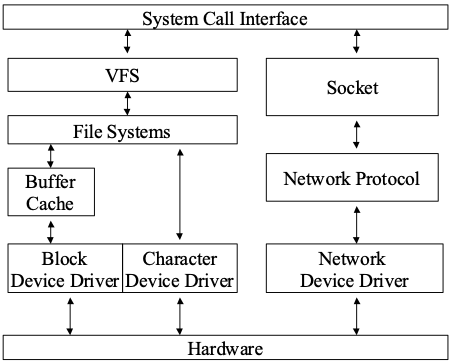
\includegraphics[width=0.3\linewidth]{figs/io-architecture.png}
%  %  \caption{xxxx}
%    \end{figure}
\end{frame}
%----------------------------------------------
% #### Linux I/O Architecture
% 
% ##### Linux I/O Architecture
% 
% ![io-architecture](figs/io-architecture.png)
% 
%----------------------------------------------
\begin{frame}[fragile]
    \frametitle{Categorizing	
 Sources	
 of	
 RISC‐V	
 Interrupts	
 }
%    \framesubtitle{xxxx}
Local	
 Interrupts	
  
    \begin{itemize}
    \item  Directly	connected	 to	 one	 hart	
    \item  No	 arbitration	 between	 harts	 to	 service	
    \item Determine	
 source	
 directly	
 through	
 xcause	
 CSR	
  
    \item  Only	 two	 standard	 local	 interrupts	 (software,	 timer)	
      
\end{itemize}
Global	
 (External)	
 Interrupts	
  
    \begin{itemize}
    \item  Routed	 via	 Platform‐Level	 Interrupt	 Controller	 (PLIC)	
    \item  PLIC	 arbitrates	 between	 multiple	 harts	 claiming	 interrupt	
    \item Read	 of	 memory‐mapped	 register	 returns	 source    
\end{itemize}
%% figure
%    \begin{figure}
%    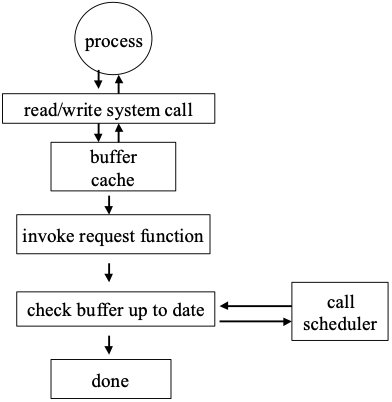
\includegraphics[width=0.47\linewidth]{figs/block-driver.png}
%  %  \caption{xxxx}
%    \end{figure}
\end{frame}
%----------------------------------------------
% ##### Block Driver
% 
% ![block-driver](figs/block-driver.png)
% 
%----------------------------------------------
\begin{frame}[fragile]
    \frametitle{machine interrupt pending CSR - mip}
%    \framesubtitle{xxxx}
    \begin{itemize}
    \item  mip reflects pending status of interrupts for hart
    \item  separate interrupts for each supported privilege level(M/H/S/U)	  
\end{itemize}
%% figure
    \begin{figure}
    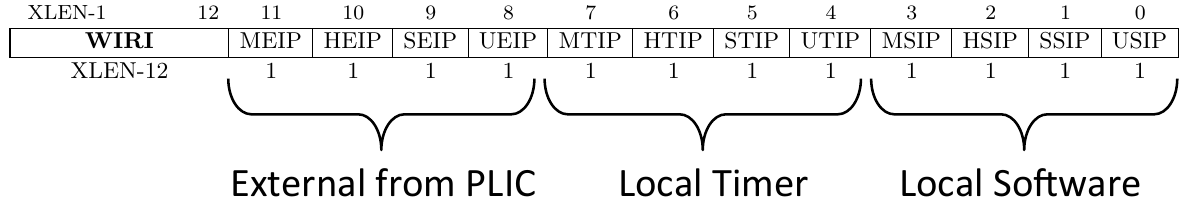
\includegraphics[width=1.\linewidth]{rv-mip.png}
  %  \caption{xxxx}
    \end{figure}
\end{frame}
%----------------------------------------------
% ##### Network Driver
% 
% ![network-driver](figs/network-driver.png)
% 
%----------------------------------------------
\subsection{Device Driver} % A subsection can be created just before a set of slides with a common theme to further break down your presentation into chunks
%----------------------------------------------
\begin{frame}[fragile]
    \frametitle{PlaCorm-­‐Level	 Interrupt	 Controller	 (PLIC)	 }
%    \framesubtitle{xxxx}
%% figure
    \begin{figure}
    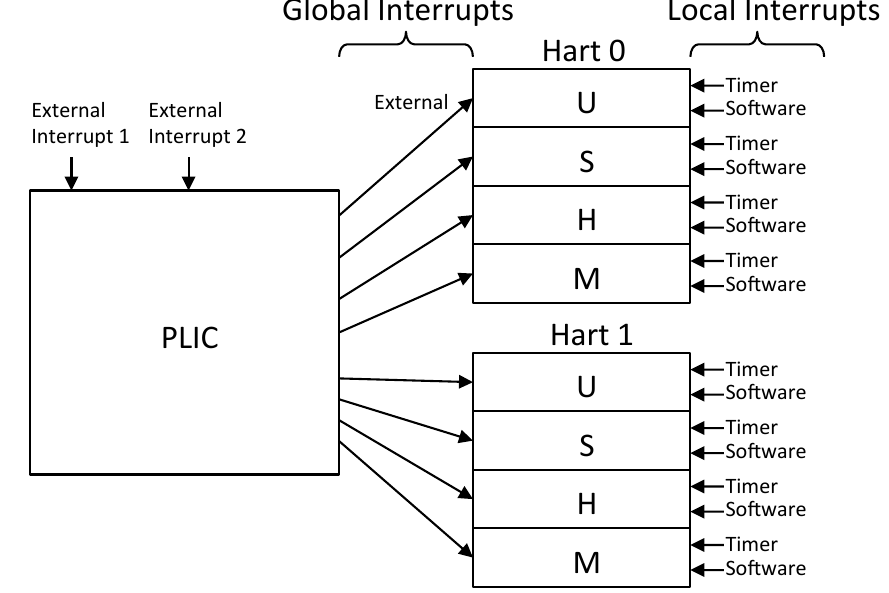
\includegraphics[width=0.7\linewidth]{figs/rv-plic.png}
  %  \caption{xxxx}
    \end{figure}
\end{frame}

%----------------------------------------------
\begin{frame}[fragile]
    \frametitle{PlaCorm-­‐Level	 Interrupt	 Controller	 (PLIC)	 }
    %    \framesubtitle{xxxx}
    %% figure
    \begin{figure}
        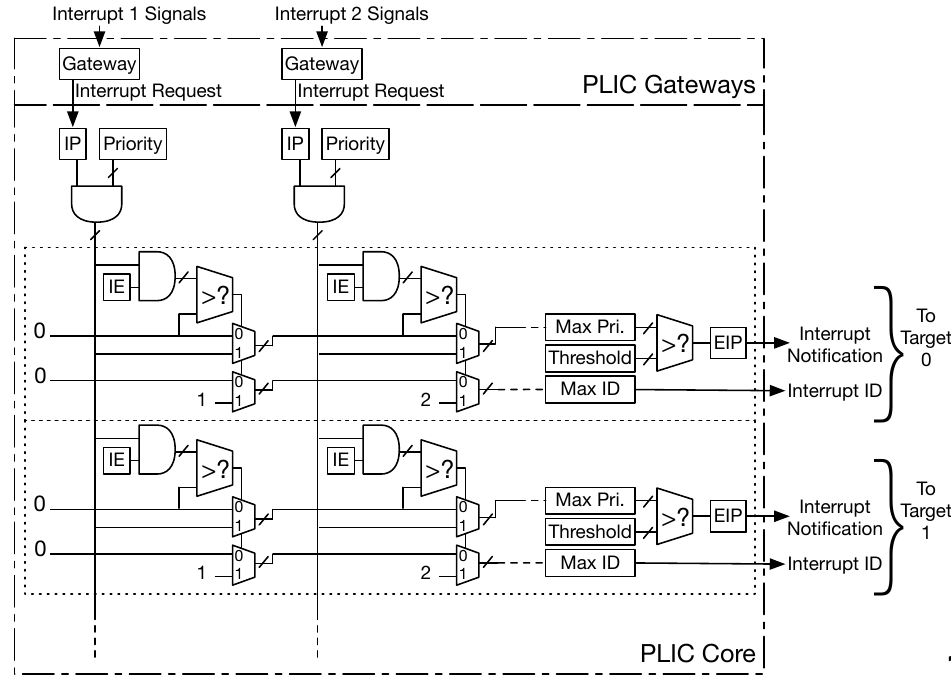
\includegraphics[width=0.6\linewidth]{figs/rv-plic-detail.png}
        %  \caption{xxxx}
    \end{figure}
\end{frame}

%----------------------------------------------
\begin{frame}[fragile]
    \frametitle{machine interrupt enable CSR - mie}
    %    \framesubtitle{xxxx}
    \begin{itemize}
        \item  mie mirrors layout of mip
        \item  provides per-interrupt enables	  
    \end{itemize}
    %% figure
    \begin{figure}
        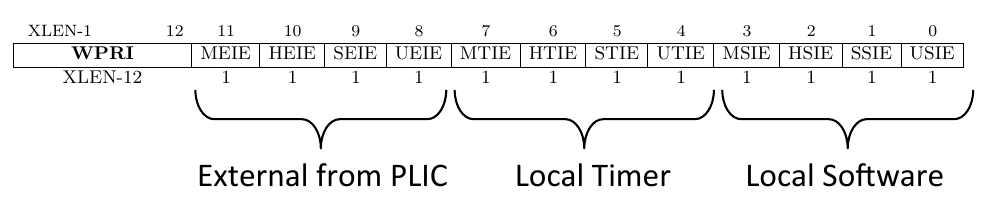
\includegraphics[width=0.9\linewidth]{rv-mie.png}
        %  \caption{xxxx}
    \end{figure}
\end{frame}
%----------------------------------------------
\begin{frame}[fragile]
    \frametitle{interrupts in mstatus}
    %    \framesubtitle{xxxx}
    \begin{itemize}
        \item  only take a pending interrupt for privilege mode x if xIE=1 and running in mode x or greater
        \item  interrupts always disabled for privileges less than current level  
    \end{itemize}
    %% figure
    \begin{figure}
        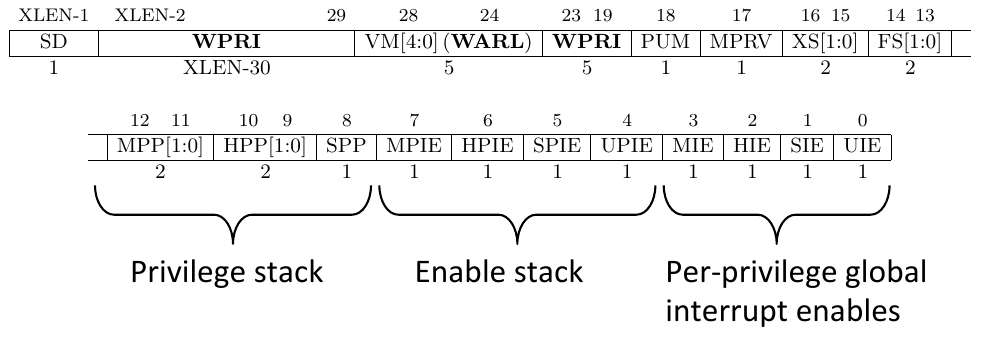
\includegraphics[width=1.\linewidth]{rv-mstatus.png}
        %  \caption{xxxx}
    \end{figure}
\end{frame}

%----------------------------------------------
\begin{frame}[fragile]
    \frametitle{interrupts related CSR}
    %    \framesubtitle{xxxx}
    中断相关的控制状态寄存器(CSR)
    \begin{itemize}
        \item mtvec(Machine Trap Vector):发生异常时处理器需要跳转到的地址
        \item mepc(Machine Exception PC):指向发生中断时的指令
        \item mie(Machine Interrupt Enable):处理器目前能处理和必须忽略的中断
        \item mip(Machine Interrupt Pending):正准备处理的中断
        \item mscratch(Machine Scratch):暂时存放一个字大小的数据
        \item mcause(Machine Cause):发生中断的种类
        \item mstatus(Machine Status):机器的状态
        \item mscratch(Machine Scratch):暂时存放一个字大小的数据
        \item S模式有异常处理CSR:sepc, stvec, scause, sscratch和sstatus,与M模式的寄存器相对应
    \end{itemize}
    指令 mret / sret : 从机器态/内核态返回前一被打断的态,同时将 pc 的值设置为 mepc/sepc
%    %% figure
%    \begin{figure}
%        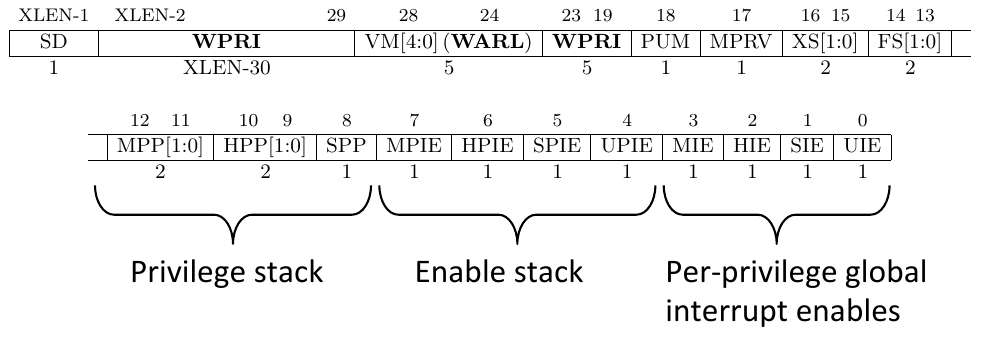
\includegraphics[width=1.\linewidth]{rv-mstatus.png}
%        %  \caption{xxxx}
%    \end{figure}
\end{frame}

%----------------------------------------------
\begin{frame}[fragile]
    \frametitle{M模式中断处理(硬件部分)}
    %    \framesubtitle{xxxx}
    \begin{itemize}
        \item 查看是否允许中断,例:如果 mstatus.MIE = 1,mie[7] = 1,且 mip[7] = 1,则可以处理机器的时钟中断
        \item 被中断的指令的PC被保存在mepc中,pc被置为mtvec。(对于中断它指向中断处理后应该恢复执行的位置)
        \item 根据中断来源设置mcause
        \item 把状态寄存器mstatus中的MIE位置零以禁用中断,并把先前的MIE值保留到MPIE中
        \item 发生中断前的权限模式保留在mstatus的MPP域中,再把权限模式更改为M
    \end{itemize}
    %    %% figure
    %    \begin{figure}
    %        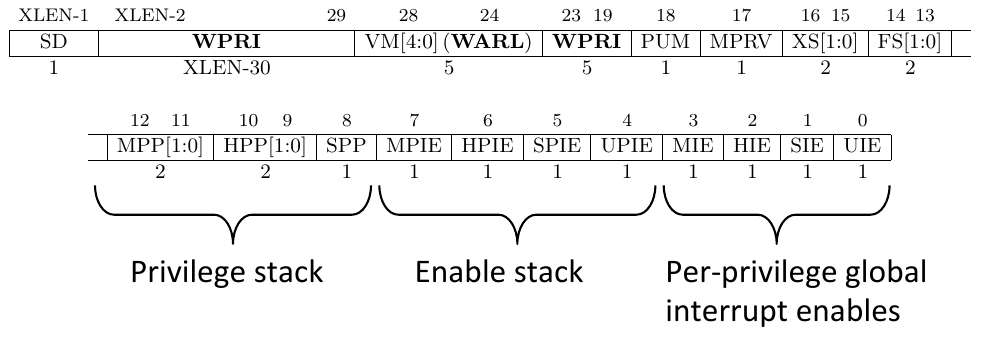
\includegraphics[width=1.\linewidth]{rv-mstatus.png}
    %        %  \caption{xxxx}
    %    \end{figure}
\end{frame}

%----------------------------------------------
\begin{frame}[fragile]
    \frametitle{有S模式的异常处理}
    %    \framesubtitle{xxxx}
    \begin{itemize}
        \item 默认情况下,所有产生的中断都使得控制权移交到M模式的异常处理程序
        \item M模式的中断处理例程可以将中断重新导向S模式,但是这些额外的操作会减慢中断的处理速度
        \item RISC-V提供一种中断委托机制,通过该机制可以选择性地将中断交给 S 模式处理,而完全绕过 M 模式
    \end{itemize}
    %    %% figure
    %    \begin{figure}
    %        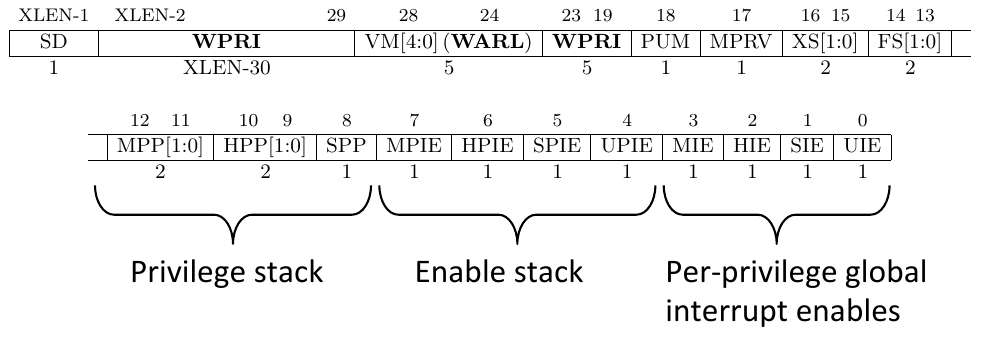
\includegraphics[width=1.\linewidth]{rv-mstatus.png}
    %        %  \caption{xxxx}
    %    \end{figure}
\end{frame}

%----------------------------------------------
\begin{frame}[fragile]
    \frametitle{中断委托寄存器}
    %    \framesubtitle{xxxx}
    \begin{itemize}
        \item mideleg (Machine Interrupt Delegation)CSR控制将哪些中断委托给S模式处理
        \item 例如mideleg[5]对应于S模式的时钟中断,如果把它置位,S模式的时钟中断将会移交S模式的中断处理例程,而不是M模式的中断处理例程
        \item 委托给S模式的任何中断都可以被S模式的软件设置为屏蔽。sie(Supervisor Interrupt Enable)和sip(Supervisor Interrupt Pending)CSR是S模式的控制状态寄存器,是mie和mip的子集。这两个寄存器和M模式下有相同的布局。sie和sip中只有与由mideleg委托的中断对应的位才能读写,没有委派的中断对应位总是0
    \end{itemize}
    %    %% figure
    %    \begin{figure}
    %        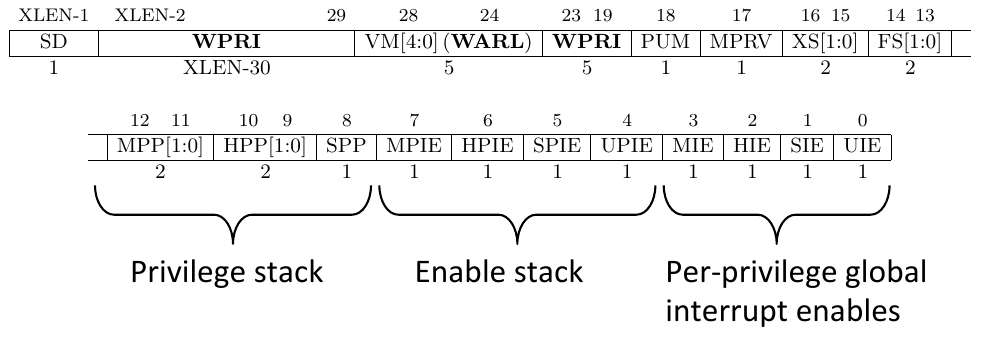
\includegraphics[width=1.\linewidth]{rv-mstatus.png}
    %        %  \caption{xxxx}
    %    \end{figure}
\end{frame}

%----------------------------------------------
\begin{frame}[fragile]
    \frametitle{S模式中断处理(硬件部分)}
    %    \framesubtitle{xxxx}
    \begin{itemize}
        \item 查看是否允许中断,例:如果 sstatus.MIE = 1,sie[7] = 1,且 sip[7] = 1,则可以处理机器的时钟中断
        \item 被中断的指令的PC被保存在sepc中,pc被置为stvec。(对于中断它指向中断处理后应该恢复执行的位置)
        \item 根据中断来源设置scause
        \item 把状态寄存器mstatus中的MIE位置零以禁用中断,并把先前的MIE值保留到MPIE中
        \item 发生中断前的权限模式保留在sstatus的SPP域中,再把权限模式更改为S
    \end{itemize}
    %    %% figure
    %    \begin{figure}
    %        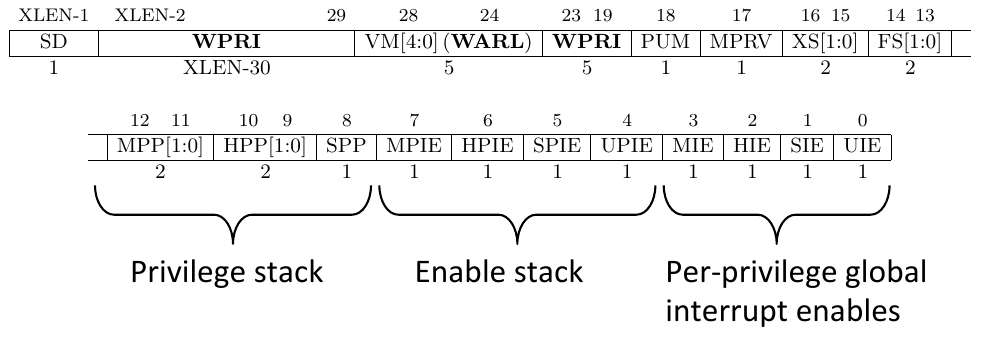
\includegraphics[width=1.\linewidth]{rv-mstatus.png}
    %        %  \caption{xxxx}
    %    \end{figure}
\end{frame}
%----------------------------------------------
\end{document}
